%!TEX root =../../course-notes.tex
% ^ leave for LaTeXTools build functionality

\begin{module}{V}{Vector Spaces}

\begin{moduleStandards}
  \item \textbf{V1: Vector Spaces.}
        Determine if a set with given operations forms a vector space.
  \item \textbf{V2: Linear Combinations.}
        Determine if a vector can be written as a linear combination of
        a given set of vectors.
  \item \textbf{V3: Spanning Sets.}
        Determine if a set of vectors spans a vector space.
  \item \textbf{V4: Subspaces.}
        Determine if a subset of a vector space is a subset or not.
\end{moduleStandards}

%!TEX root =../../course-notes.tex
% ^ leave for LaTeXTools build functionality

\begin{readinessAssuranceOutcomes}
\item Add Euclidean vectors and multiply Euclidean vectors by scalars.
\item Add complex numbers and multiply complex numbers by scalars.
\item Add polynomials and multiply polynomials by scalars.
\item Perform basic manipulations of augmented matrices and linear
systems \standardList{E1,E2,E3}.
\end{readinessAssuranceOutcomes}

\begin{readinessAssuranceResources}
\item \url{https://www.khanacademy.org/math/precalculus/vectors-precalc/vector-addition-subtraction/v/adding-and-subtracting-vectors}
\item \url{https://www.khanacademy.org/math/precalculus/vectors-precalc/combined-vector-operations/v/combined-vector-operations-example}
\item \url{https://www.khanacademy.org/math/precalculus/imaginary-and-complex-numbers/adding-and-subtracting-complex-numbers/v/adding-complex-numbers}
\item \url{https://www.khanacademy.org/math/algebra/introduction-to-polynomial-expressions/adding-and-subtracting-polynomials/v/adding-and-subtracting-polynomials-1}
\end{readinessAssuranceResources}




\begin{readinessAssuranceTest}

\item Simplify the following vector expression.
  \[
  2
  \begin{bmatrix}
    3 \\ -1 \\ 0
  \end{bmatrix}-
  3
  \begin{bmatrix}
    0 \\ 2 \\ 1
  \end{bmatrix}
  \]

\begin{multicols}{4}
\begin{readinessAssuranceTestChoices}
\item \(
        \begin{bmatrix}
          0 \\ 4 \\ -8
        \end{bmatrix}
      \)
\item \(
        \begin{bmatrix}
          6 \\ -8 \\ -3
        \end{bmatrix}
      \) % correct
\item \(
        \begin{bmatrix}
          3 \\ 2 \\ -5
        \end{bmatrix}
      \)
\item \(
        \begin{bmatrix}
          -2 \\ 0 \\ 1
        \end{bmatrix}
      \)
\end{readinessAssuranceTestChoices}
\end{multicols}

\item Simplify the following vector expression.
  \[
  2\left(
  \begin{bmatrix}
    1 \\ 1 \\ -1
  \end{bmatrix}+
  \begin{bmatrix}
    -1 \\ 1 \\ -3
  \end{bmatrix}\right)
  \]

\begin{multicols}{4}
\begin{readinessAssuranceTestChoices}
\item \(
        \begin{bmatrix}
          0 \\ 4 \\ -8
        \end{bmatrix}
      \) % correct
\item \(
        \begin{bmatrix}
          6 \\ -8 \\ -3
        \end{bmatrix}
      \)
\item \(
        \begin{bmatrix}
          3 \\ 2 \\ -5
        \end{bmatrix}
      \)
\item \(
        \begin{bmatrix}
          -2 \\ 0 \\ 1
        \end{bmatrix}
      \)
\end{readinessAssuranceTestChoices}
\end{multicols}

\item Simplify the complex number expression
      \(-4(3-2i)+2(5+i)\).

\begin{multicols}{4}
\begin{readinessAssuranceTestChoices}
\item \(3-7i\)
\item \(4+i\)
\item \(-2+10i\) % correct
\item \(-1-5i\)
\end{readinessAssuranceTestChoices}
\end{multicols}

\item Which of these complex numbers might be represented
      by the following vector
      plotted on the complex plane (where the horizontal axis gives the
      real part and the vertical axis gives the imaginary part)?

      \begin{center}
        \begin{tikzpicture}[scale=0.25]
        \draw[thin,gray,<->] (-5,0) -- (5,0);
        \draw[thin,gray,<->] (0,-5) -- (0,5);
        \draw[thick,blue,->] (0,0) -- (-2,3);
        \end{tikzpicture}
      \end{center}

\begin{multicols}{4}
\begin{readinessAssuranceTestChoices}
\item \(5+i\)
\item \(-3-9i\)
\item \(-2+3i\) % correct
\item \(4i\)
\end{readinessAssuranceTestChoices}
\end{multicols}

\item Simplify \(3f(x)-2g(x)\) where
      \(f(x)=7-x^2\) and
      \(g(x)=2x^3+x-1\).

\begin{multicols}{4}
\begin{readinessAssuranceTestChoices}
\item \(x^3+4x-5\)
\item \(-4x^3-3x^2-2x+23\) % correct
\item \(3x^3+5x^2-3x+17\)
\item \(-x^3+19x^2-4\)
\end{readinessAssuranceTestChoices}
\end{multicols}

\item Express the following system of linear equations as an augmented matrix.
\begin{alignat*}{5}
  x_1 &\,+\,& 2x_2 &\, \,&     &\,-\,&  x_4 &\,=\,& 3 \\
      &\, \,&      &\, \,& x_3 &\,+\,& 4x_4 &\,=\,& -2
\end{alignat*}

\begin{multicols}{4}
\begin{readinessAssuranceTestChoices}
\item \(
      \begin{bmatrix}[c|c]
        1 & 0 \\
        2 & 0 \\
        0 & 1 \\
        -1 & 4 \\
        -2 & 3
      \end{bmatrix}
    \)
\item \(
      \begin{bmatrix}[cccc|c]
        1 & 2 & 0 & -1 & 3 \\
        0 & 0 & 1 & 4 & -2
      \end{bmatrix}
    \) % correct
    \item \(
          \begin{bmatrix}[c|c]
            1 & 2 \\
            0 & -1 \\
            3 & 0 \\
            0 & 1 \\
            4 & -2
          \end{bmatrix}
        \)
\item \(
      \begin{bmatrix}[cccc|c]
        1 & 2 & 1 & 4 & 3 \\
        -2 & 1 & 3 & 4 & 5
      \end{bmatrix}
    \)
\end{readinessAssuranceTestChoices}
\end{multicols}

\item Which of the following matrices is equivalent to the following matrix?
  \[
    \begin{bmatrix}[cc|c]
      1 & 2 & 3 \\
      0 & 4 & -1 \\
      2 & 3 & 2 \\
    \end{bmatrix}
  \]
  (Hint: The correct answer was obtained from a single row operation.)

  \begin{multicols}{4}
  \begin{readinessAssuranceTestChoices}
  \item
    \(
      \begin{bmatrix}[cc|c]
        1 & 2 & 3 \\
        0 & 4 & -1 \\
        0 & 0 & 1 \\
      \end{bmatrix}
    \)
  \item
    \(
      \begin{bmatrix}[cc|c]
        1 & 2 & 3 \\
        1 & 3 & 4 \\
        2 & 3 & 2 \\
      \end{bmatrix}
    \)
  \item
    \(
      \begin{bmatrix}[cc|c]
        1 & 2 & 3 \\
        0 & 1 & 1 \\
        2 & 3 & 2 \\
      \end{bmatrix}
    \)
  \item
    \(
      \begin{bmatrix}[cc|c]
        1 & 2 & 3 \\
        0 & 4 & -1 \\
        0 & -1 & -4 \\
      \end{bmatrix}
    \) % correct
  \end{readinessAssuranceTestChoices}
  \end{multicols}

\item Find
  \(\RREF
    \begin{bmatrix}[cc|c]
      1 & 2 & 3 \\
      0 & 4 & -1 \\
      2 & 3 & 2 \\
    \end{bmatrix}
  \).

  \begin{multicols}{4}
  \begin{readinessAssuranceTestChoices}
  \item
    \(
      \begin{bmatrix}[cc|c]
        1 & 0 & 3 \\
        0 & 1 & -1 \\
        0 & 0 & 0 \\
      \end{bmatrix}
    \)
  \item
    \(
      \begin{bmatrix}[cc|c]
        1 & 2 & 3 \\
        1 & 3 & 4 \\
        0 & 0 & 0 \\
      \end{bmatrix}
    \)
  \item
    \(
      \begin{bmatrix}[cc|c]
        1 & 2 & 3 \\
        0 & 1 & 1 \\
        0 & 0 & 0 \\
      \end{bmatrix}
    \)
  \item
    \(
      \begin{bmatrix}[cc|c]
        1 & 0 & 0 \\
        0 & 1 & 0 \\
        0 & 0 & 1 \\
      \end{bmatrix}
    \) % correct
  \end{readinessAssuranceTestChoices}
  \end{multicols}

  \item Solve the following system of linear equations.
  \begin{alignat*}{4}
    2x_1 &\,+\,& x_2 &\,+\,& 4x_3 &\,=\,& 0 \\
     x_1 &\,+\,& x_2 &\,+\,&  x_3 &\,=\,& 1 \\
   -3x_1 &\,+\,& 4x_2 &\,+\,& x_3 &\,=\,& -7 \\
  \end{alignat*}

  \begin{multicols}{2}
  \begin{readinessAssuranceTestChoices}
  \item \(
          \begin{bmatrix}
            x_1 \\ x_2 \\ x_3
          \end{bmatrix}=
          \begin{bmatrix}
            2 \\ 0 \\ -1
          \end{bmatrix}
        \) % correct
  \item \(
          \begin{bmatrix}
            x_1 \\ x_2 \\ x_3
          \end{bmatrix}=
          \begin{bmatrix}
            1 \\ -6 \\ 1
          \end{bmatrix}
        \)
  \item \(
          \begin{bmatrix}
            x_1 \\ x_2 \\ x_3
          \end{bmatrix}=
          \begin{bmatrix}
            1 \\ -2 \\ 1
          \end{bmatrix}+
          a
          \begin{bmatrix}
            1 \\ 0 \\ 3
          \end{bmatrix}
        \) for all real numbers \(a\)
  \item No solutions
  \end{readinessAssuranceTestChoices}
  \end{multicols}

  \item Solve the following system of linear equations.
  \begin{alignat*}{4}
    2x_1 &\,+\,& x_2 &\,+\,& 4x_3 &\,=\,& 0 \\
     x_1 &\,+\,& x_2 &\,+\,&  x_3 &\,=\,& 0 \\
  \end{alignat*}

  \begin{multicols}{2}
  \begin{readinessAssuranceTestChoices}
  \item \(
          \begin{bmatrix}
            x_1 \\ x_2 \\ x_3
          \end{bmatrix}=
          \begin{bmatrix}
            4 \\ 1 \\ -5
          \end{bmatrix}
        \)
  \item \(
          \begin{bmatrix}
            x_1 \\ x_2 \\ x_3
          \end{bmatrix}=
          \begin{bmatrix}
            1 \\ 2 \\ -1
          \end{bmatrix}
        \)
  \item \(
          \begin{bmatrix}
            x_1 \\ x_2 \\ x_3
          \end{bmatrix}=
          a
          \begin{bmatrix}
            -3 \\ 2 \\ 1
          \end{bmatrix}
        \) for all real numbers \(a\) % correct
  \item No solutions
  \end{readinessAssuranceTestChoices}
  \end{multicols}



\end{readinessAssuranceTest}

%!TEX root =../../course-notes.tex
% ^ leave for LaTeXTools build functionality

\begin{applicationActivities}{Day 1}

\begin{activity}{15}
Let \(\vect u=\begin{bmatrix} u_1 \\ u_2 \end{bmatrix}\),
\(\vect v=\begin{bmatrix} v_1 \\ v_2 \end{bmatrix}\), and
\(\vect w=\begin{bmatrix} w_1 \\ w_2 \end{bmatrix}\).
Rewrite the following proofs about two-dimensional Euclidean vector addition,
filling in the missing information.
\begin{enumerate}
  \item Euclidean vector addition is \textbf{well-defined}.

        \textbf{Proof:} \(\vect u+\vect v=?\). Since this is a Euclidean
        vector, addition is well-defined. \(\square\)
  \item Euclidean vector addition is \textbf{associative}.

        \textbf{Proof:} \(\vect u+(\vect v+\vect w)=\,?\) and
        \((\vect u+\vect v)+\vect w=\,?\). Since both expressions are equal,
        addition is associative. \(\square\)
  \item Euclidean vector addition is \textbf{commutative}.

        \textbf{Proof:} \(\vect u+\vect v=\,?\) and
        \(\vect v+\vect u=\,?\). Since both expressions are equal,
        addition is commutative. \(\square\)
  \item There exists an \textbf{additive identity} for Euclidean vector
        addition.

        \textbf{Proof:} Let \(\vect 0=\,?\). Since
        \(\vect v+\vect 0=\,?=\vect v\), \(\vect 0\) is an identity. \(\square\)
  \item Every Euclidean vector has an \textbf{additive inverse}.

        \textbf{Proof:} Let \(-\vect v=\,?\). Since
        \(\vect v+(-\vect v)=\,?=\vect 0\), \(-\vect v\) is an inverse
        for \(\vect v\). \(\square\)
\end{enumerate}
\end{activity}

\begin{activity}{15}
Let \(\vect u=\begin{bmatrix} u_1 \\ u_2 \end{bmatrix}\) and
\(\vect v=\begin{bmatrix} v_1 \\ v_2 \end{bmatrix}\), and let \(a,b\) be
scalar numbers.
Rewrite the following proofs about scalar multiplication of
two-dimensional Euclidean vectors,
filling in the missing information.
\begin{enumerate}
  \item Scalar multiplication of Euclidean vectors is \textbf{well-defined}.

        \textbf{Proof:} \(a\vect v=?\). Since this is a Euclidean
        vector, scalar multiplication is well-defined. \(\square\)
  \item Scalar multiplication of Euclidean vectors is \textbf{compatible}.

        \textbf{Proof:} \(a(b\vect v)=\,?\) and
        \((ab)\vect v=\,?\). Since both expressions are equal,
        scalar multiplication is compatible. \(\square\)
  \item Scalar multiplication of Euclidean vectors
        \textbf{distributes scalars}.

        \textbf{Proof:} \(a(\vect u+\vect v)=\,?\) and
        \(a\vect u+a\vect v=\,?\). Since both expressions are equal,
        scalars distribute. \(\square\)
  \item Scalar multiplication of Euclidean vectors
        \textbf{distributes vectors}.

        \textbf{Proof:} \((a+b)\vect v=\,?\) and
        \(a\vect v+b\vect v=\,?\). Since both expressions are equal,
        vectors distribute. \(\square\)
  \item The scalar \(1\) is a \textbf{multiplicative identity} for the
        scalar multiplication of Euclidean vectors.

        \textbf{Proof:} Since
        \(1\vect v=\,?=\vect v\), \(1\) is an identity. \(\square\)
\end{enumerate}
\end{activity}

\begin{definition}
  A \textbf{vector space} \(V\) is any collection of mathematical objects with
  associated addition and scalar multiplication operations that satisfy
  the following properties. Let \(\vect u,\vect v,\vect w\) belong to \(V\),
  and let \(a,b\) be scalar numbers.
  \begin{multicols}{2}
  \begin{itemize}
    \item \textbf{Well-defined addition.}

          \(\vect v+\vect w\) belongs to \(V\).
    \item \textbf{Associative addition.}

          \(\vect u+(\vect v+\vect w)=
          (\vect u+\vect v)+\vect w\).
    \item \textbf{Commutative addition.}

          \(\vect u+\vect v=
          \vect v+\vect u\).
    \item \textbf{Additive identity.}

          There exists some \(\vect 0\) in \(V\)
          where \(\vect v+\vect 0=\vect v\).
    \item \textbf{Additive identity.}

          There exists some \(-\vect v\) in \(V\)
          where \(\vect v+(-\vect v)=\vect 0\).
    \item \textbf{Well-defined scalar multipication.}

          \(a\vect v\) belongs to
          \(V\).
    \item \textbf{Compatible scalar multipication.}

          \(a(b\vect v)=(ab)\vect v\).
    \item \textbf{Scalar distribution.}

          \(a(\vect u+\vect v)=a\vect u+a\vect v\).
    \item \textbf{Vector distribution.}

          \((a+b)\vect v=a\vect v+b\vect v\).
    \item \textbf{Scalar multiplication identity.}

          \(1\vect v=\vect v\).
  \end{itemize}
  \end{multicols}
\end{definition}

\begin{definition}
  The most important examples of vector spaces are the \term{Euclidean
  vector spaces} \(\IR^n\), but there are other examples as well.
\end{definition}

\begin{activity}{15}
  Assuming the usual definitions of addition and scalar multiplication,
  label each of the following sets as a \textbf{valid} or \textbf{non-valid}
  vector space. If the set is not a valid vector space, give an example of
  a vector space property that fails to hold.
  \begin{multicols}{2}
  \begin{enumerate}
    \item \(\left\{
    \begin{bmatrix}
      v_1\\v_2\\v_3\\v_4
    \end{bmatrix}:v_i\text{ is an integer}\right\}\)
    \item \(\left\{
      a+bi
      :a,b\text{ are real numbers}\right\}\)
    \item \(\left\{
      x^2+bx+c
      :b,c\text{ are positive}\right\}\)
  \end{enumerate}
  \end{multicols}
\end{activity}



\end{applicationActivities}

%!TEX root =../../course-notes.tex
% ^ leave for LaTeXTools build functionality

\begin{applicationActivities}{2}{8}

\begin{remark}
  The following sets are examples of vector spaces, with the usual/natural
  operations for addition and scalar multiplication.
  \begin{itemize}
    \item \(\IR^n\): Euclidean vectors with \(n\) components.
    \item \(\IR^\infty\): Sequences of real numbers \((v_1,v_2,\dots)\).
    \item \(\IR^{m\times n}\): Matrices of real numbers with \(m\) rows and
          \(n\) columns.
    \item \(\IC\): Complex numbers.
    \item \(\P^n\): Polynomials of degree \(n\) or less.
    \item \(\P\): Polynomials of any degree.
    \item \(C(\IR)\): Real-valued continuous functions.
  \end{itemize}
\end{remark}

\begin{activity}{15}
  Let \(V=\{(a,b):a,b\text{ are real numbers}\}\), where \((a_1,b_1)+(a_2,b_2)=
  (a_1+b_1+a_2+b_2,b_1^2+b_2^2)\) and \(c(a,b)=(a^c,b+c)\). Show that
  this is not a vector space by finding a counterexample
  that does not satisfy one of the vector space properties.

  \vectorSpaceProperties
\end{activity}

\begin{definition}
  A \term{linear combination} of a set of vectors
  \(\{\vect v_1,\vect v_2,\dots,\vect v_m\}\) is given by
  \(c_1\vect v_1+c_2\vect v_2+\dots+c_m\vect v_m\) for any choice of
  scalar multiples \(c_1,c_2,\dots,c_m\).
\end{definition}

\begin{definition}
  The \term{span} of a set of vectors is the collection of all linear
  combinations of that set:
  \[
    \vspan\{\vect v_1,\vect v_2,\dots,\vect v_m\} =
    \{c_1\vect v_1+c_2\vect v_2+\dots+c_m\vect v_m :
    c_i\text{ is a real number}\}
  \]
\end{definition}

\begin{activity}{10}
  Consider \(\vspan\left\{\begin{bmatrix}1\\2\end{bmatrix}\right\}\).
  \begin{subactivity}
    Sketch
    \(c\begin{bmatrix}1\\2\end{bmatrix}\) in the \(xy\) plane
    for \(c=1,3,0,-2\).
  \end{subactivity}
  \begin{subactivity}
    Sketch a representation of all the vectors given by
    \(\vspan\left\{\begin{bmatrix}1\\2\end{bmatrix}\right\}\)
    in the \(xy\) plane.
  \end{subactivity}
\end{activity}

\begin{activity}{10}
  Consider \(\vspan\left\{\begin{bmatrix}1\\2\end{bmatrix},
  \begin{bmatrix}-1\\1\end{bmatrix}\right\}\).
  \begin{subactivity}
    Sketch
    \(c_1\begin{bmatrix}1\\2\end{bmatrix}+
    c_2\begin{bmatrix}-1\\1\end{bmatrix}\) in the \(xy\) plane
    for \(\begin{bmatrix}c_1\\c_2\end{bmatrix}=
    \begin{bmatrix}1\\0\end{bmatrix},
    \begin{bmatrix}0\\1\end{bmatrix},
    \begin{bmatrix}2\\0\end{bmatrix},
    \begin{bmatrix}2\\1\end{bmatrix}\).
  \end{subactivity}
  \begin{subactivity}
    Sketch a representation of all the vectors given by
    \(\vspan\left\{\begin{bmatrix}1\\2\end{bmatrix},
     \begin{bmatrix}-1\\1\end{bmatrix}\right\}\)
    in the \(xy\) plane.
  \end{subactivity}
\end{activity}

\begin{activity}{5}
    Sketch a representation of all the vectors given by
    \(\vspan\left\{\begin{bmatrix}6\\-4\end{bmatrix},
     \begin{bmatrix}-2\\3\end{bmatrix}\right\}\)
    in the \(xy\) plane.
\end{activity}

% \begin{activity}{10} % Motivate with vectors first.
%   Consider the following linear system.
%     \begin{alignat*}{3}
%        x_1 &\,-\,&  x_2 &\,=\,& -1 \\
%            &\,-\,& 3x_2 &\,=\,& -6 \\
%      -3x_1 &\,+\,& 2x_2 &\,=\,&  1
%     \end{alignat*}
%   \begin{subactivity}
%     Solve this system by using a calculator to find
%     \[\RREF
%       \begin{bmatrix}[cc|c]
%         1 & -1 & -1 \\
%         0 & -3 & -6 \\
%         -3 & 2 & 1
%       \end{bmatrix}
%     \]
%   \end{subactivity}
%   \begin{subactivity}
%     Given this solution, does
%     \(\begin{bmatrix}-1\\-6\\1\end{bmatrix}\) belong to
%     \(\vspan\left\{\begin{bmatrix}1\\0\\-3\end{bmatrix},
%     \begin{bmatrix}-1\\-3\\2\end{bmatrix}\right\}\)?
%   \end{subactivity}
% \end{activity}

\begin{activity}{10}
  The vector
  \(\begin{bmatrix}-1\\-6\\1\end{bmatrix}\) belongs to
  \(\vspan\left\{\begin{bmatrix}1\\0\\-3\end{bmatrix},
  \begin{bmatrix}-1\\-3\\2\end{bmatrix}\right\}\) exactly when
  the vector equation
  \(x_1\begin{bmatrix}1\\0\\-3\end{bmatrix}+
  x_2\begin{bmatrix}-1\\-3\\2\end{bmatrix}
  =\begin{bmatrix}-1\\-6\\1\end{bmatrix}\) holds for some scalars
  \(x_1,x_2\).
  \begin{subactivity}
    Reinterpret this vector equation as a system of linear equations.
  \end{subactivity}
    % \begin{alignat*}{3}
    %    x_1 &\,-\,&  x_2 &\,=\,& -1 \\
    %        &\,-\,& 3x_2 &\,=\,& -6 \\
    %  -3x_1 &\,+\,& 2x_2 &\,=\,&  1
    % \end{alignat*}
  \begin{subactivity}
    Solve this system. (From now on, feel free to use a calculator
    to solve linear systems.)
    % \[\RREF
    %   \begin{bmatrix}[cc|c]
    %     1 & -1 & -1 \\
    %     0 & -3 & -6 \\
    %     -3 & 2 & 1
    %   \end{bmatrix}
    % \]
  \end{subactivity}
  \begin{subactivity}
    Given this solution, does
    \(\begin{bmatrix}-1\\-6\\1\end{bmatrix}\) belong to
    \(\vspan\left\{\begin{bmatrix}1\\0\\-3\end{bmatrix},
    \begin{bmatrix}-1\\-3\\2\end{bmatrix}\right\}\)?
  \end{subactivity}
\end{activity}


\end{applicationActivities}

%!TEX root =../../course-notes.tex
% ^ leave for LaTeXTools build functionality

\begin{applicationActivities}{Day 3}


\begin{observation}
  So far we've only discussed linear combinations of Euclidean vectors.
  Fortunately, many vector spaces of interest can be reinterpreted as an
  \term{isomorphic} Euclidean space \(\IR^n\); that is, a Euclidean space
  that mirrors the behavior of the vector space exactly.
\end{observation}

\begin{activity}{5}
  We previously checked that \(\begin{bmatrix}3\\-2\\1\end{bmatrix}\)
  does not belong to
  \(\vspan\left\{\begin{bmatrix}1\\0\\-3\end{bmatrix},
  \begin{bmatrix}-1\\-3\\2\end{bmatrix}\right\}\).
  Does \(f(x)=3x^2-2x+1\) belong to
  \(\vspan\{x^2-3,-x^2-3x+2\}\)?
\end{activity}

\begin{activity}{10}
  Does the matrix \(\begin{bmatrix}6&3\\2&-1\end{bmatrix}\) belong to
  \(\vspan\left\{\begin{bmatrix}1&0\\0&-1\end{bmatrix},
  \begin{bmatrix}4&3\\2&1\end{bmatrix}\right\}\)?
\end{activity}

\begin{activity}{10}
  Does the complex number \(2i\) belong to
  \(\vspan\{-3+i,6-2i\}\)?
\end{activity}

\begin{definition}
  A subset of a vector space is called a \term{subspace} if it contains
  all of its own linear combinations. Every subspace is itself a vector space.
\end{definition}

\begin{fact}
  If \(S\) is a subset of a vector space \(V\), then
  \(\vspan S\) is a subspace of \(V\).
\end{fact}

\begin{remark}
  To prove that a subset is a subspace, you only need to check that
  \(c\vect v+d\vect w\) belongs to the subset for any choice of
  vectors \(\vect v,\vect w\) from the subset and any real scalars \(c,d\).
\end{remark}

\begin{activity}{5}
  Prove that \(P=\{ax^2+b:a,b\text{ are both real numbers}\}\) is a subspace
  of the vector space of all degree-two polynomials by showing that
  \(c(a_1x^2+b_1)+d(a_2x^2+b_2)\) belongs to \(P\).
\end{activity}

\begin{activity}{10}
  Consider the subset of \(\IR^2\) where at least one coordinate on
  each vector is \(0\).
  \begin{center}
    \begin{tikzpicture}[scale=0.25]
    \draw[thin,gray,<->] (-5,0) -- (5,0);
    \draw[thin,gray,<->] (0,-5) -- (0,5);
    \draw[thick,blue] (-4.8,0) -- (4.8,0);
    \draw[thick,blue] (0,-4.8) -- (0,4.8);
    \end{tikzpicture}
  \end{center}
  \begin{subactivity}
  Sketch a picture that demonstrates why this is not a subspace of \(\IR^2\).
  \end{subactivity}
  \begin{subactivity}
    Define an explicit example of a linear combination
    \(c\begin{bmatrix}v_1\\v_2\end{bmatrix}+
    d\begin{bmatrix}w_1\\w_2\end{bmatrix}\) that does not
    belong to this subset.
  \end{subactivity}
\end{activity}

\begin{fact}
  Suppose a subset \(S\) of \(V\) is isomorphic to another vector space
  \(W\).
  Then \(S\) is a subspace of \(V\).
\end{fact}

\begin{activity}{10}
  Show that the upper triangular matrices
  \[U^{2\times 2}=
    \left\{
    \begin{bmatrix}a&b\\0&c\end{bmatrix} :
    a,b,c\text{ are real numbers}
    \right\}
  \]
  form a subspace of \(\IR^{2\times 2}\) by finding a Euclidean
  space isomorphic to \(U^{2\times 2}\).
\end{activity}



\end{applicationActivities}

%!TEX root =../../course-notes.tex
% ^ leave for LaTeXTools build functionality

\begin{applicationActivities}{4}{10}

\begin{fact}
  At least \(n\) vectors are required to span \(\IR^n\).

  \begin{center}
  \begin{tikzpicture}[scale=0.5]
    \draw[<->] (-4,0) -- (4,0);
    \draw[<->] (0,-4) -- (0,4);
    \draw[blue!50] (2,-4) -- (-2,4);
    \draw[thick,blue,->] (0,0) -- (1,-2);
  \end{tikzpicture}
  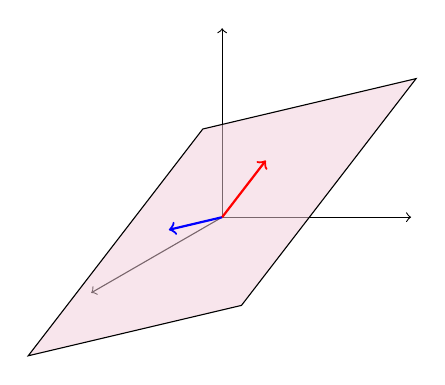
\begin{tikzpicture}[x={(210:0.8cm)}, y={(0:1cm)}, z={(90:1cm)},scale=0.4]
    \draw[->] (0,0,0) -- (6,0,0);
    \draw[->] (0,0,0) -- (0,6,0);
    \draw[->] (0,0,0) -- (0,0,6);
    \draw[fill=purple!20,fill opacity=0.5]
      (-2,-2,2) -- (6,-2,-2) -- (2,2,-2) -- (-6,2,2) -- (-2,-2,2);
    \draw[thick,blue,->] (0,0,0) -- (1,-1,0);
    \draw[thick,red,->] (0,0,0) -- (-2,0,1);
  \end{tikzpicture}
  \end{center}
\end{fact}

\begin{activity}{10}
  Choose a vector \(\begin{bmatrix}a\\b\\c\end{bmatrix}\)
  in \(\IR^3\) that is not in
  \(\vspan\left\{\begin{bmatrix}1\\-1\\0\end{bmatrix},
  \begin{bmatrix}-2\\0\\1\end{bmatrix}\right\}\) by ensuring
  \(\begin{bmatrix}[cc|c]1&-2&a\\-1&0&b\\0&1&c\end{bmatrix}\sim
  \begin{bmatrix}[cc|c]1&0&0\\0&1&0\\0&0&1\end{bmatrix}\).
  (Why does this work?)
\end{activity}

\begin{fact}
  The set \(\{\vect v_1,\dots,\vect v_m\}\) fails to span all of \(\IR^n\)
  exactly when \(\RREF[\vect v_1\,\dots\,\vect v_m]\) has a row of zeros:
  \[\begin{bmatrix}[cc]1&-2\\-1&0\\0&1\end{bmatrix}\sim
  \begin{bmatrix}[cc]1&0\\0&1\\0&0\end{bmatrix}\Rightarrow
  \begin{bmatrix}[cc|c]1&-2&a\\-1&0&b\\0&1&c\end{bmatrix}\sim
  \begin{bmatrix}[cc|c]1&0&0\\0&1&0\\0&0&1\end{bmatrix}\]
\end{fact}

\begin{activity}{5}
  Consider the set of vectors \(S=\left\{
  \begin{bmatrix}2\\3\\0\\-1\end{bmatrix},
  \begin{bmatrix}1\\-4\\3\\0\end{bmatrix},
  \begin{bmatrix}2\\0\\0\\3\end{bmatrix},
  \begin{bmatrix}0\\3\\5\\7\end{bmatrix},
  \begin{bmatrix}3\\13\\7\\16\end{bmatrix}
  \right\}
  \).
  Does
  \(\IR^4=\vspan S\)?
  % \begin{subactivity}
  % Find a linear combination of vectors in \(S\) that equals
  % \(\begin{bmatrix}-1\\10\\7\\14\end{bmatrix}\).
  % \end{subactivity}
\end{activity}

\begin{activity}{10}
  Consider the set of third-degree polynomials \[S=\left\{
  2x^3+3x^2-1,
  2x^3+3,
  3x^3+13x^2+7x+16,
  -x^3+10x^2+7x+14,
  4x^3+3x^2+2
  \right\}
  .\]
  Does
  \(\P^3=\vspan S\)?
  % \begin{subactivity}
  % Find a vector in \(\IR^4\) that is not in \(\vspan S\).
  % \end{subactivity}
\end{activity}

\begin{definition}
  A subset of a vector space is called a \term{subspace} if it is
  itself a vector space.
\end{definition}

\begin{fact}
  If \(S\) is a subset of a vector space \(V\), then
  \(\vspan S\) is a subspace of \(V\).
\end{fact}

\begin{remark}
  To prove that a subset is a subspace, you need only verify that
  \(c\vect v+d\vect w\) belongs to the subset for any choice of
  vectors \(\vect v,\vect w\) from the subset and any real scalars \(c,d\).
\end{remark}

\begin{activity}{5}
  Prove that \(P=\{ax^2+b:a,b\text{ are both real numbers}\}\) is a subspace
  of the vector space of all degree-two polynomials by showing that
  \(c(a_1x^2+b_1)+d(a_2x^2+b_2)\) belongs to \(P\).
\end{activity}

\begin{activity}{10}
  Consider the subset of \(\IR^2\) where at least one coordinate of
  each vector is \(0\).
  \begin{center}
    \begin{tikzpicture}[scale=0.25]
    \draw[thin,gray,<->] (-5,0) -- (5,0);
    \draw[thin,gray,<->] (0,-5) -- (0,5);
    \draw[thick,blue] (-4.8,0) -- (4.8,0);
    \draw[thick,blue] (0,-4.8) -- (0,4.8);
    \end{tikzpicture}
  \end{center}
  % \begin{subactivity}
    Find a linear combination
    \(c\vect v+
    d\vect w\) that does not
    belong to this subset.
  % \end{subactivity}
  \begin{TBLnote}
    Use this linear combination to sketch a picture
    illustrating why this subset is not
    a subspace.
  \end{TBLnote}
\end{activity}

\begin{fact}
  Suppose a subset \(S\) of \(V\) is isomorphic to another vector space
  \(W\).
  Then \(S\) is a subspace of \(V\).
\end{fact}

\begin{activity}{5}
  Show that the set of \(2\times 2\) matrices
  \[S=
    \left\{
    \begin{bmatrix}a&b\\-b&-a\end{bmatrix} :
    a,b\text{ are real numbers}
    \right\}
  \]
  is a subspace of \(\IR^{2\times 2}\) by selecting a Euclidean
  space isomorphic to \(S\).
\end{activity}



\end{applicationActivities}


\end{module}
